\section{Results}
\label{sec:results}

\subsection{Simulation}

Fig. \ref{fig:initialgeometry} shows snapshots of the simulation of an initial test geometry at initial and final time steps. 

\begin{figure}[h!]
    \centering
    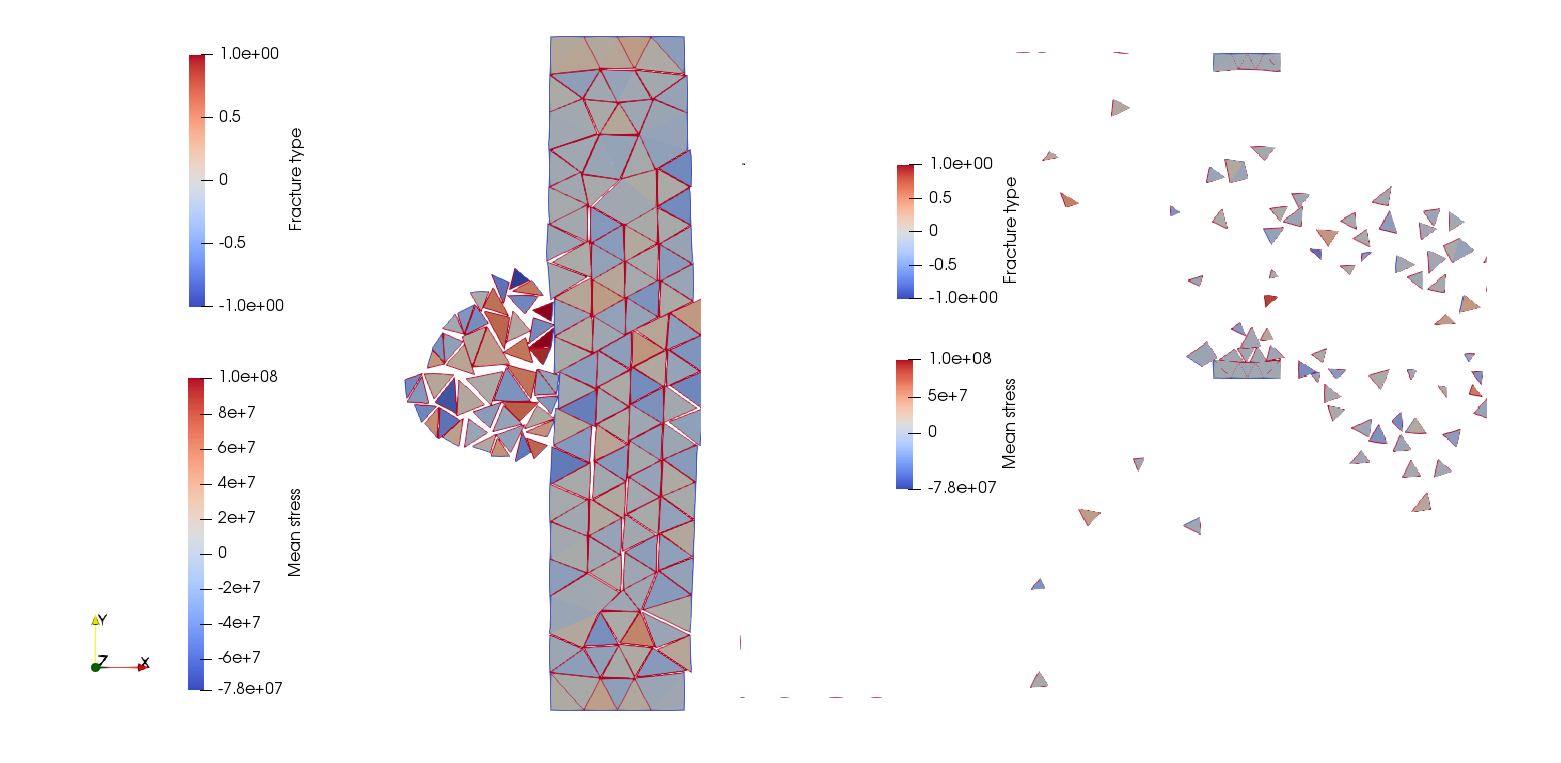
\includegraphics[width=\columnwidth]{initialgeom}
    \caption{Snapshots of simulation setup of a test geometry, at initial and final time steps.}
    \label{fig:initialgeometry}
\end{figure}

Fig. \ref{fig:finalgeometry} shows a snapshot of the simulation of the final geometry at the final time step. 

\begin{figure}[h!]
    \centering
    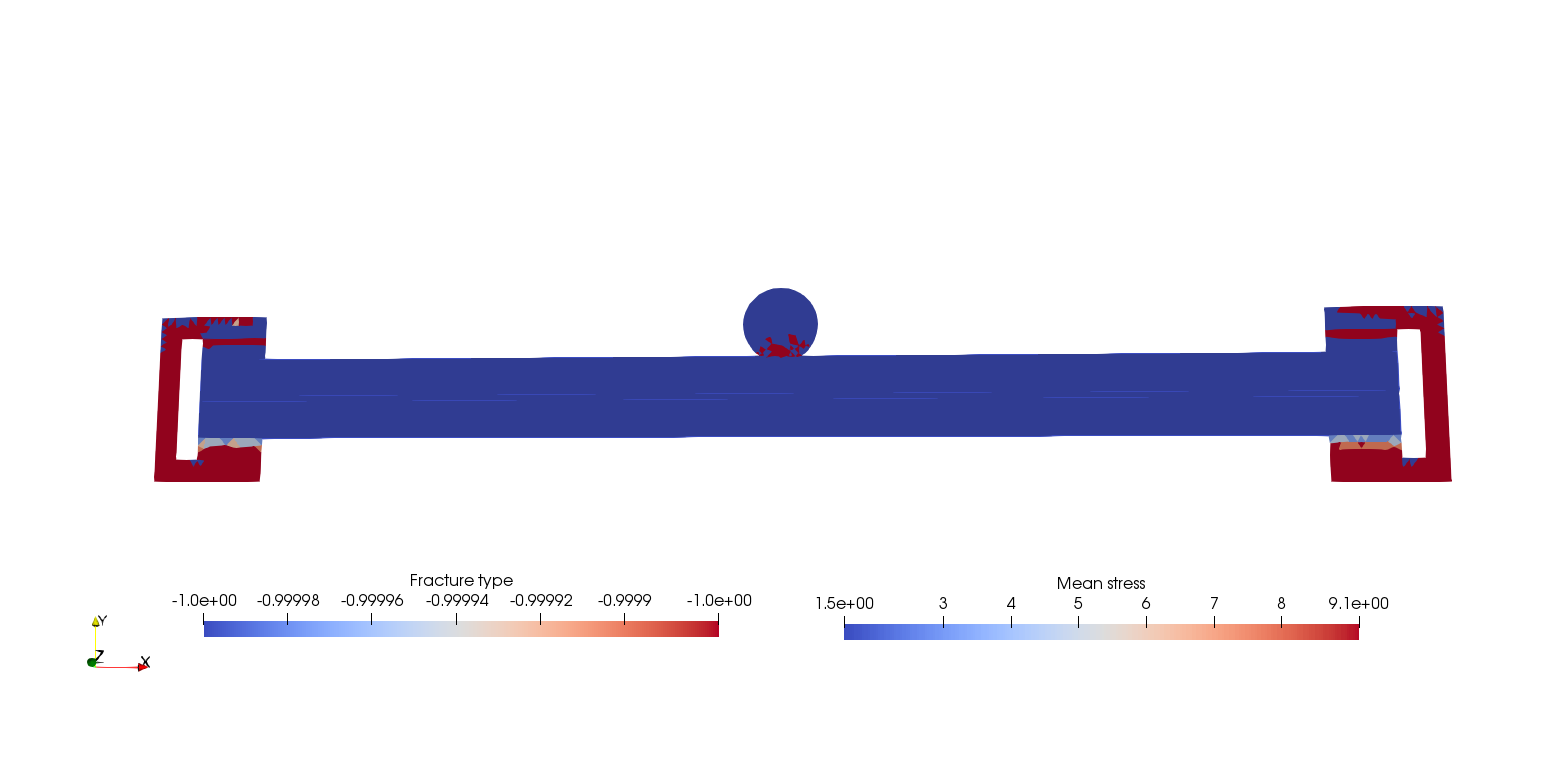
\includegraphics[width=\columnwidth]{finalgeometrie}
    \caption{Snapshot of simulation setup as described in section \ref{sec:NumericalModelApproach} at final time step}
    \label{fig:finalgeometry}
\end{figure}

\subsection{VTK implementation}

\begin{listing}[p!]
\xmlminted{vtk_legacy.vtu}
\caption{Example \texttt{VTK} legacy ascii encoded file}
\label{lst:vtklegacy}
\end{listing}

\begin{longlisting}
\xmlminted{vtk_xml_inline.vtu}
\caption{Example \texttt{VTK XML} file with \texttt{b64} inline encoding}
\label{lst:vtkxmlinline}
\end{longlisting}

\bigbreak
An example \texttt{VTK} legacy output file is given by List. \ref{lst:vtklegacy}. An example \texttt{VTK XML b64} inline encoded output file is given by List. \ref{lst:vtkxmlinline}.